\documentclass[9pt,twocolumn,twoside]{../../styles/osajnl}
\usepackage{fancyvrb}
\journal{i524} 

\title{Apache Lucene}

\author[1,*, +]{Roy Choudhury, Sabyasachi}

\affil[1]{School of Informatics and Computing, Bloomington, IN 47408, U.S.A.}

\affil[*]{Corresponding authors: sabyroyc@indiana.edu}

\affil[+]{HID - S17-IO-3015}

\dates{project-000, \today}

\ociscodes{Search Engine Library, Lucene}

% replace this with your url in github/gitlab
\doi{\url{https://github.com/sabyasachi087/sp17-i524/tree/master/paper1/S17-IO-3015/report.pdf}}


\begin{abstract}
This paper gives an overview of Apache Lucene. We will go through the basic architecture and functionality of the library. We will see the advantages and downfalls of Lucene and conclude on its implementation.
\newline
\end{abstract}

\setboolean{displaycopyright}{true}

\begin{document}

\maketitle

\section{Introduction}

Apache Lucene is a search library that enables search facility to any application. Although it was initially written in Java but has been ported to many languages chiefly C-Sharp, c/c++ , Python etc. It is an active open source project and under Apache License. Its latest release is \href{http://lucene.apache.org/core/6_4_1/index.html}{6.4.1}. It is important that we must understand that Lucene is just a search library and cannot handle other related stuffs like crawling, document filtering , administration etc.

\section{Concepts}
To understand the purpose of Lucene we have to be familiar with two terms, one is "Information Overload" and "Information Retrieval"\cite{wiki-ir}. The term information overload means, difficulty that one can have in making decisions, because of the presence of too much of information. In another words, "Information Overload" can occur if the rate of feed/input into a system exceeds its processing capabilities. Imagine the situation of current world. We are living in the world where data has reached volume of zeta bytes. To extract some insight , first step is to collect all related data. This is known as information retrieval(IR). IR is the task of collecting relevant information from collection of data resources scattered across devices. Now with the above understanding we can say Lucene is a scalable Information Retrieval library.

\subsection{Lucene and Search Engine}
Google has set some base expectations for search engines, which if not available can cause dissatisfaction for the users. For example spell checker and response time of <= 1 second. Lucene should be able to met those expectations or else its not worth. But Lucene is not a full fledged search engine rather its a tool kit to achieve so. So lets jot down the steps for any search engine 

Module  : Raw Content -> Gather Data -> Analyze -> Index ->  Query Support 
UseCase : User query -> Search Engine -> Build Query -> Extract Information from indexed data

\section{Architecture}
Figure 1 explains a basic architecture of Lucene

\begin{figure}[htbp]
\centering
\fbox{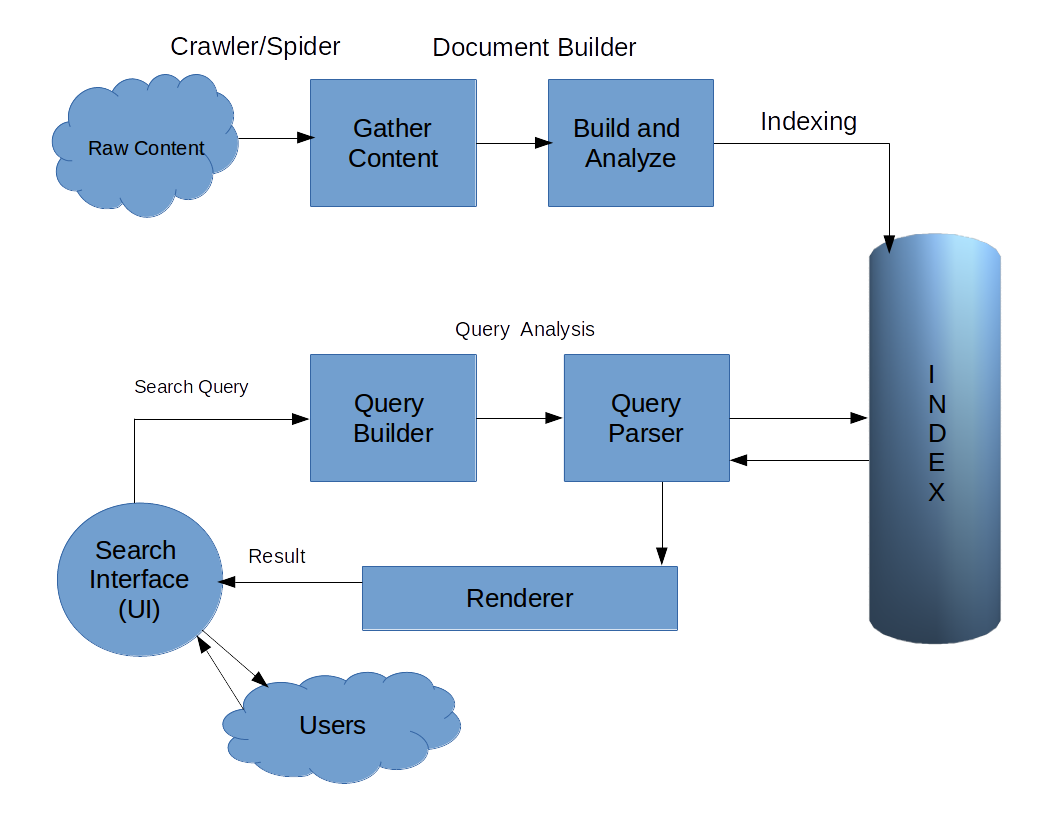
\includegraphics[width=\linewidth]{images/Apache_Lucene_Architecure.png}}
\caption{Apache Lucene Architecture.}
\label{fig:lucene-data-flow}
\end{figure}

Lucene library is compact and does not have any external dependencies. But it can be plugged with other libraries for building a search engine. Fig 1\cite{lucene-book} shows process flow of Lucene. On a high level , data collected from different sources are analyzed and converted into smaller chunks. These are known as documents. Documents are text entries and from these text entries Lucene performs indexing and store it in local disk for future reference. The next step is to handle the search query from users. Lucene has a query parser to understand the query and search the index for the correct or relevant match. If found, returns the document back. We will elaborate the flow beneath.

\section{Lucene Components}

\subsection{Document Analysis and Indexing}
Data or contents which are available in different format and location needs to be gathered. This process is typically done by a crawler/spider. Core Lucene does not have these capabilities and can be considered to be a pre-requisite for Lucene to implement.Two of the crawler that are build on Lucene are \href{http://lucene.apache.org/solr}{Solr} and \href{http://lucene.apache.org/nutch}{Nutch}. Once the data is collected , document has to be constructed from the contents. The design of constructing documents has to be decided by the user and implemented within Lucene. Lucene provides an API for building documents but logic has to be provided by the implementation layer. Lucene also does not provide any API for document filtering. But yet again we have Tika , which is built on Lucene, can be used for this purpose. But we cannot index the document yet. We cannot index the raw content within the document directly. Before that , we need to break the content into smaller chunks known as tokens. Each token is map to a "word". Analysis includes handling compound words, spell check, typo correction injection of synonyms, etc. Lucene has built in support of list of analyzers which gives a fine grain control over analysis. Once tokenization is done , now its time for indexing. Lucene takes care all of the need to cater this step. An API has been provide for this purpose, but has to be implemented carefully as the searching will solely depend upon how well the indexing has been done.


\subsection{Searching}
It is a look up process within the index to extract the most relevant (matching) documents. It is based on two matrices i.e. Precision and Recall. Recall measures how well the system finds the relevant documents and Precision measures the filtering out the irrelevant one. Lucene offers benchmarking technique for measuring these matrices. User Interface (UI) is equally important for a search application as that is what the end user is going to use. Lucene does not provide any UI support. When user inputs the search query the first step is to build the query. User inputs are human readable and need further processing before it can be used within the application. Lucene provides a powerful parser for this job known as QueryParser. Even it is default state it does the job pretty clean but often needs extension as per some advance requirements. Finally hitting the search query to index. Almost everything about this is catered by Lucene and also provide option for extension. It finds the result and returns all relevant document objects. Its the responsibility of the UI to render the results correctly.

\section{Advance Usages}
Lucene has some advance feature for administration and analytics. For example Lucene allows to configure the RAM buffer size , re-indexing ,commit and purge scheduler. It allows some fault tolerance mechanism in case a newly added document failed to index. Related to analytics it also provides some meta information regarding the search queries it receives and the results it renders. For example which kind of query are run , query hitting lowest relevance , query having no results and so on. One big problem within the list of advance usages that Lucene does not support is "Scaling". Scaling in terms of both through put and processing speed. In a clustered environment this is quiet an important part as data and resource all are distributed. But both Solr and Nutch provides data partitioning and sharding to achieve higher throughput if not speed. Elastic search is another option which is based upon Lucene and provides distributed computing.


\section{Conclusion}
Lucene is the standard library for search applications. It can be compared with 'C' (language) of computing which is small and powerful but requires much more effort to build an entire application. It must be remembered that Lucene is just a library which sits at the core of the functionality but it needs much more than that to build an application. Elastic Search , Solr and Nutch which are based on Lucene are preferred tools in terms of building enterprise level search engines. 

\section{Reading Sources}

\begin{itemize}
\item Lucene In Action \cite{lucene-book} provides a startup guide to
learn, build and implement search engines based on Lucene 
\item Lucene at tutorial point \cite{www-lucene-tp} provides introduction
 to Lucene Library.
\end{itemize}



\section*{Acknowledgements}

Thanking Prof. Gregor von Laszewski for his technical help and support.


% Bibliography

\bibliography{references}

\end{document}
